% 图 22.3 —— 由 `checks/emit_hand.py` 自动拼出（probe 精测 + prims2 图元分解）
%%
% ⚠ 这是**稿子不是成品**：跑 `checks/checkhand.py 22.3` 看指标 + 看叠合图。
%%
%% ⚠ 待核：
%   · 本图 probe 报出阴影族 1 个 —— **本脚本不生成阴影**（要照原书手写）；prims2 的 strokes 里可能含阴影线，核对时留意别画重
%   · 可疑字形 1 项（空心圈 ⊙ 常被认成字母 o）—— 见文件末
%%
\documentclass[12pt]{standalone}
\usepackage{fontspec}
\setsansfont{Arial}
\newfontfamily\mfallback{DejaVu Sans}
\usepackage{tikz}
\begin{document}
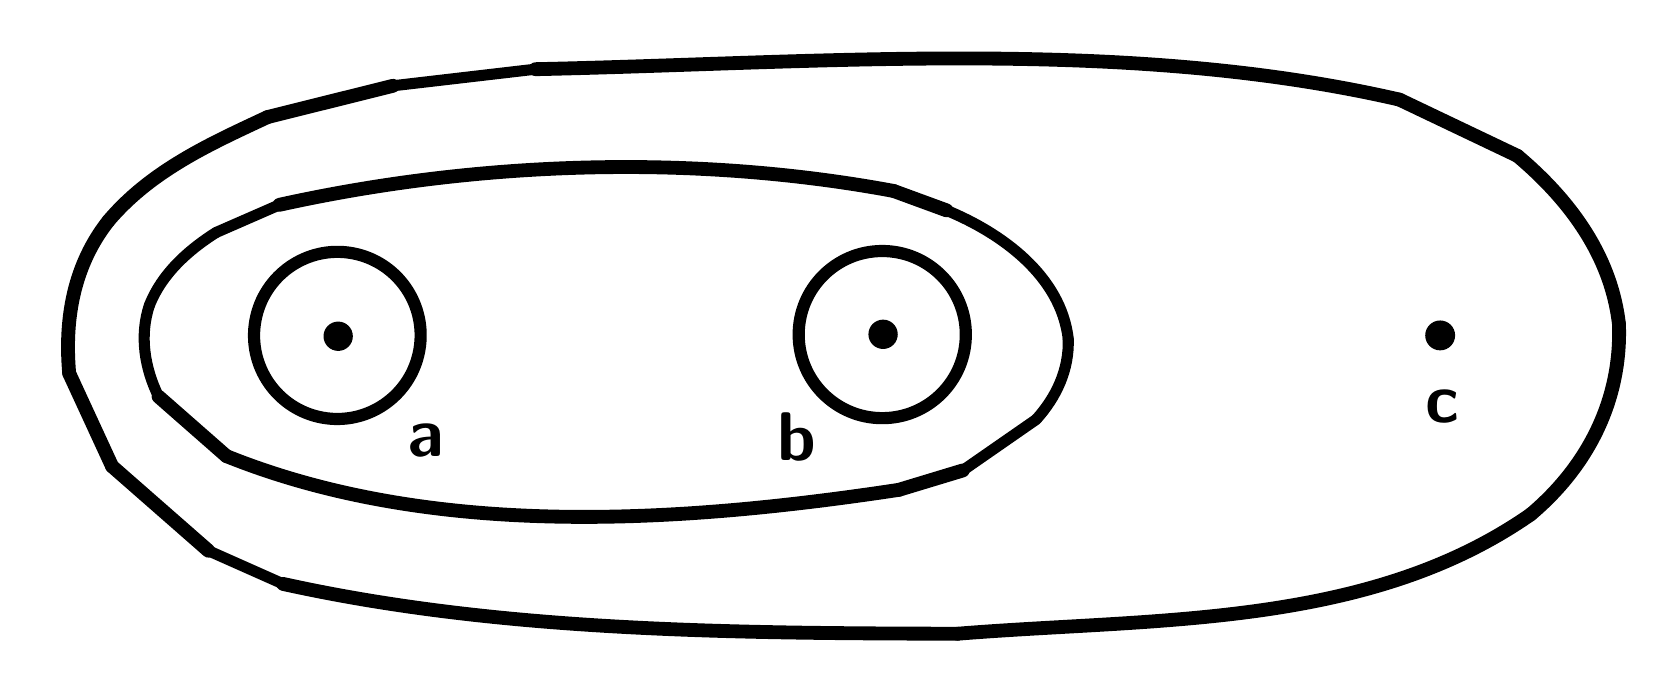
\begin{tikzpicture}[x=1pt, y=-1pt, line width=4.4pt, line cap=round, line join=round]

  %% ════ 填充区（prims2 的 fills）════

  %% ════ 直线段（prims2 的 strokes）════
  \draw[line width=4.0pt] (92.3,201.0) -- (65.3,189.0);
  \draw[line width=5.0pt] (65.3,189.0) -- (30.5,158.5);
  \draw[line width=5.0pt] (30.5,158.5) -- (15.0,124.9);
  \draw[line width=5.0pt] (86.7,32.3) -- (132.0,21.0);
  \draw[line width=4.0pt] (132.0,21.0) -- (183.5,15.0);
  \draw[line width=5.0pt] (495.7,26.0) -- (538.3,46.3);
  \draw[line width=5.0pt] (332.0,66.0) -- (312.9,59.0);
  \draw[line width=4.0pt] (91.0,64.0) -- (68.1,74.0);
  \draw[line width=5.0pt] (47.3,133.3) -- (71.8,154.8);
  \draw[line width=5.0pt] (314.8,167.0) -- (337.9,160.0);
  \draw[line width=4.0pt] (337.9,160.0) -- (364.4,141.6);

  %% ════ 曲线（prims2 的 curves —— 三段式，坐标同为 (y,x)）════
  \draw[line width=5.0pt] (336.0,219.0) .. controls (253.5,218.8) and (170.1,218.2) .. (92.3,201.0);
  \draw[line width=5.0pt] (15.0,124.9) .. controls (13.2,104.5) and (16.9,85.4) .. (29.2,69.8);
  \draw[line width=5.0pt] (29.2,69.8) .. controls (44.8,51.4) and (66.4,41.8) .. (86.7,32.3);
  \draw[line width=5.0pt] (183.5,15.0) .. controls (287.5,12.8) and (396.6,3.2) .. (495.7,26.0);
  \draw[line width=5.0pt] (538.3,46.3) .. controls (557.7,62.6) and (572.2,82.8) .. (575.0,107.1);
  \draw[line width=5.0pt] (575.0,107.1) .. controls (576.0,134.0) and (564.2,158.1) .. (543.1,175.9);
  \draw[line width=5.0pt] (543.1,175.9) .. controls (484.0,217.1) and (407.5,213.2) .. (336.0,219.0);
  \draw[line width=5.0pt] (312.9,59.0) .. controls (240.2,45.5) and (162.0,48.3) .. (91.0,64.0);
  \draw[line width=4.0pt] (68.1,74.0) .. controls (58.0,80.4) and (48.5,88.9) .. (44.0,100.3);
  \draw[line width=4.0pt] (44.0,100.3) .. controls (40.3,111.3) and (42.3,123.1) .. (47.3,133.3);
  \draw[line width=5.0pt] (71.8,154.8) .. controls (146.5,184.9) and (235.3,179.0) .. (314.8,167.0);
  \draw[line width=4.0pt] (364.4,141.6) .. controls (371.7,133.5) and (376.4,123.6) .. (376.0,112.4);
  \draw[line width=4.0pt] (376.0,112.4) .. controls (373.3,89.6) and (351.9,74.2) .. (332.0,66.0);

  %% ════ 圆 / 椭圆（probe 精测）════
  \draw (308.8,110.9) circle (30.2);
  \draw[rotate around={169.6:(111.9,111.2)}] (111.9,111.2) ellipse (30.1 and 30.2);

  %% ════ 实心点 ════
  \fill (309.1,110.8) circle (5.3);
  \fill (510.4,111.2) circle (5.4);
  \fill (112.2,111.5) circle (5.3);

  %% ════ 标签（probe 直接给的 \node 行）════
  %% ⚠ 全部补了 fill=white：文字在最上层，否则与曲线交叉干扰
     \node[anchor=center,inner sep=0pt,fill=white,font=\fontsize{30.5}{38.1}\selectfont] at (511.3,137.0) {\textsf{\textbf{\textit{c}}}};   % box(503,127,15,17)
     \node[anchor=center,inner sep=0pt,fill=white,font=\fontsize{30.7}{38.3}\selectfont] at (277.8,147.8) {\textsf{\textbf{\textit{b}}}};   % box(268,135,17,23)
     \node[anchor=center,inner sep=0pt,fill=white,font=\fontsize{32.0}{40.0}\selectfont] at (144.1,149.1) {\textsf{\textbf{\textit{a}}}};   % box(135,139,16,17)

  % 钉死画布：否则超出的图元/控制点会把页面撑大，1:1 回比就失准
  \pgfresetboundingbox
  \path[use as bounding box] (0,0) rectangle (585,227);
\end{tikzpicture}
\end{document}

% ⚠ 待核清单（probe 拿不准，人眼过一遍）：
%   · 未识别/跳过：⑤ 跳过/未识别的字形
